\documentclass[a4paper,reqno]{amsart}
\usepackage{amssymb}
\usepackage{amsmath}
\usepackage{tikz}

\begin{document}

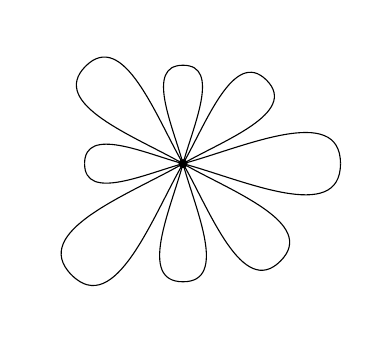
\begin{tikzpicture}
    \draw[fill] (0,0) circle(0.05);
    \foreach \ph in {0,225}{
        \begin{scope}[rotate=\ph]
        \draw (0,0) to[out={-15}, in={180+90}] (2,0);
        \draw (0,0) to[out={+15}, in={180-90}] (2,0);
        \end{scope}
    }
    \foreach \ph in {90,180}{
        \begin{scope}[rotate=\ph]
        \draw (0,0) to[out={-15}, in={180+90}] (1.25,0);
        \draw (0,0) to[out={+15}, in={180-90}] (1.25,0);
        \end{scope}
    }
    \foreach \ph in {45,270}{
        \begin{scope}[rotate=\ph]
        \draw (0,0) to[out={-15}, in={180+90}] (1.5,0);
        \draw (0,0) to[out={+15}, in={180-90}] (1.5,0);
        \end{scope}
    }
    \foreach \ph in {135,315}{
        \begin{scope}[rotate=\ph]
        \draw (0,0) to[out={-15}, in={180+90}] (1.75,0);
        \draw (0,0) to[out={+15}, in={180-90}] (1.75,0);
        \end{scope}
    }
  \end{tikzpicture}

\end{document}